\newcommand{\prompttag}[1]{\textcolor{blue}{\texttt{<|#1|>}}}

\section{Model Training Details}\label{ch2:sec:training}

% To enhance the model’s capabilities in economic and financial analysis, we employed a 2-Stage training approach combining Supervised Fine-Tuning (SFT) and Group Relative Policy Optimization (GRPO) for Reinforcement Learning (RL). 
% [Codex 修改版] 2026-02-26: 统一用 two-step/Step 1/Step 2 描述核心训练流程。
% [CH2-036][Original Start]
% To enhance the model’s capabilities in economic and financial analysis, we employ a two-step post-training approach that combines Supervised Fine-Tuning (SFT) with Reinforcement Learning (RL) via Group Relative Policy Optimization (GRPO).
% [CH2-036][Original End]
To improve macro-financial analytical performance, we use a two-step post-training pipeline: Supervised Fine-Tuning (SFT) followed by Reinforcement Learning (RL) with Group Relative Policy Optimization (GRPO).

% [CH2-037][Original Start]
% The initial stage, SFT, leverages a high-quality Question-Answer (Q\&A) dataset to train the model to generate outputs that closely align with reference answers. Given that the model is pre-trained on general-purpose textual data, SFT serves to guide the model in structuring its analysis based on economic and financial indicators. Moreover, SFT benefits from a clearly defined loss function, which facilitates stable convergence and efficient training. However, this approach has limitations, the model may primarily learn to mimic training examples, reducing its ability to generalize beyond the dataset. Additionally, there is a risk of overfitting, as the model may memorize specific phrasing or stylistic patterns from the training data, thereby limiting its creativity and adaptability. To mitigate these risks, we trained the model for only a few epochs during the SFT phase.
% [CH2-037][Original End]
In Step 1, SFT uses high-quality question--answer data to align model outputs with reference analyses. Because the base model is pre-trained on general-domain corpora, SFT provides domain adaptation toward structured economic and financial reasoning. SFT also offers stable optimization through a well-defined supervised loss. Its main risk is overfitting to stylistic patterns in the training corpus, so we limit the number of SFT epochs.


% Following SFT, in the second stage, we applied GRPO to further fine-tune the model. GRPO is a Reinforcement Learning (RL) technique that enables unsupervised training by allowing the model to self-optimize based on defined reward functions. Unlike SFT, RL supports flexible reward structures that can be adjusted to dynamically shape the model's behavior toward desired outcomes. However, RL is computationally intensive, as reward calculation is non-trivial and often model-based (e.g. LLM-as-Judge (\cite{zheng2024judging})). Furthermore, policy gradient methods in RL may introduce training instability, such as sudden drops in generation quality. To manage this, we firstly choose GRPO (\cite{shao2024deepseekmath}) as our RL training method, which reduce the computational cost by removing the reward model in the traditional RL framework (e.g. Proximal Policy Optimization (PPO, \cite{schulman2017proximal})). Additionally, we limited the GRPO training to one epoch following SFT, thereby striking a balance between enhancing reasoning capabilities and maintaining training stability.
% [Codex 修改版] 2026-02-26
% [CH2-038][Original Start]
% In Step 2, we apply GRPO to further fine-tune the model via reinforcement learning. GRPO is an on-policy RL method that allows the model to optimize against reward signals without requiring token-level reference answers. Unlike SFT, RL supports flexible reward structures (e.g., LLM-as-Judge scoring; \cite{zheng2024judging}) that can directly shape reasoning behavior. To manage the computational and stability challenges of policy-gradient training, we adopt GRPO (\cite{shao2024deepseekmath}), which reduces cost by avoiding an explicit reward model as in traditional PPO-style pipelines. In our experiments, GRPO is run for a limited number of epochs after SFT to balance reasoning improvement with training stability.
% [CH2-038][Original End]
In Step 2, GRPO further refines reasoning behavior through reward optimization. Unlike SFT, RL does not require token-level references and can directly optimize policy behavior under task-specific reward signals (e.g., LLM-as-Judge scores; \cite{zheng2024judging}). We use GRPO (\cite{shao2024deepseekmath}) to reduce the computational burden associated with traditional PPO-style pipelines and run it for a limited number of epochs after SFT to maintain stability.


% [CH2-039][Original Start]
% Following this training, the model is expected to demonstrate strong capabilities in conducting detailed economic and financial analysis, forecasting, and making monetary policy recommendations based on structured input data.
% [CH2-039][Original End]
After this two-step training, the model is expected to produce stronger data-grounded macro-financial analysis and more coherent policy-relevant reasoning from structured inputs.
% To evaluate its effectiveness, we applied the model to two downstream tasks: (1) synthetic FOMC Minutes generation and (2) Federal Funds Rate (FFR) prediction.


% In summarize, Our overall training framework consists of two stages. \textit{Stage 1} functions as a ``pre-training'' phase for downstream applications, aiming to enhance the model's domain-specific proficiency in economics and finance, as opposed to general-purpose language tasks. \textit{Stage 2} focuses on task-specific fine-tuning based on the representations and capabilities developed in Stage 1. This phase is designed to explore the model's ability to simulate domain-specific reasoning and decision-making. Figure~\ref{fig:ch2:training_process} demonstrates our training process for this research.

% In summarize, our overall training framework consists of two stages. \textit{Stage 1} involves a Supervised Fine-Tuning process, aiming to enhance the model's domain-specific proficiency in economics and finance. \textit{Stage 2} focuses on enhancing the reasoning capacity by guiding the model maximize the given reward signals via Group Relative Policy Optimization. Figure~\ref{fig:ch2:training_process} demonstrates our training process for this research.

% In summary, our overall training framework consists of two stages. \textit{Stage 1} involves \textbf{Supervised Fine-Tuning (SFT)}, which aims to enhance the model’s domain-specific understanding of economics and finance. \textit{Stage 2} focuses on strengthening the model’s reasoning capability by optimizing reward-guided learning through \textbf{Group Relative Policy Optimization (GRPO)}. The entire training workflow is illustrated in Figure~\ref{fig:ch2:training_process}.
% [Codex 修改版] 2026-02-26
% [CH2-040][Original Start]
% In summary, our overall training framework consists of two steps. \textit{Step 1} applies \textbf{Supervised Fine-Tuning (SFT)} to enhance domain-specific understanding and structured analysis generation. \textit{Step 2} applies \textbf{Group Relative Policy Optimization (GRPO)} to strengthen reasoning behavior through reward-guided learning. The overall workflow is illustrated in Figure~\ref{fig:ch2:training_process}.
% [CH2-040][Original End]
In summary, Step 1 (SFT) performs domain adaptation for structured analysis, and Step 2 (GRPO) improves reasoning quality through reward-guided optimization. Figure~\ref{fig:ch2:training_process} summarizes the workflow.




\begin{figure}
    \centering
    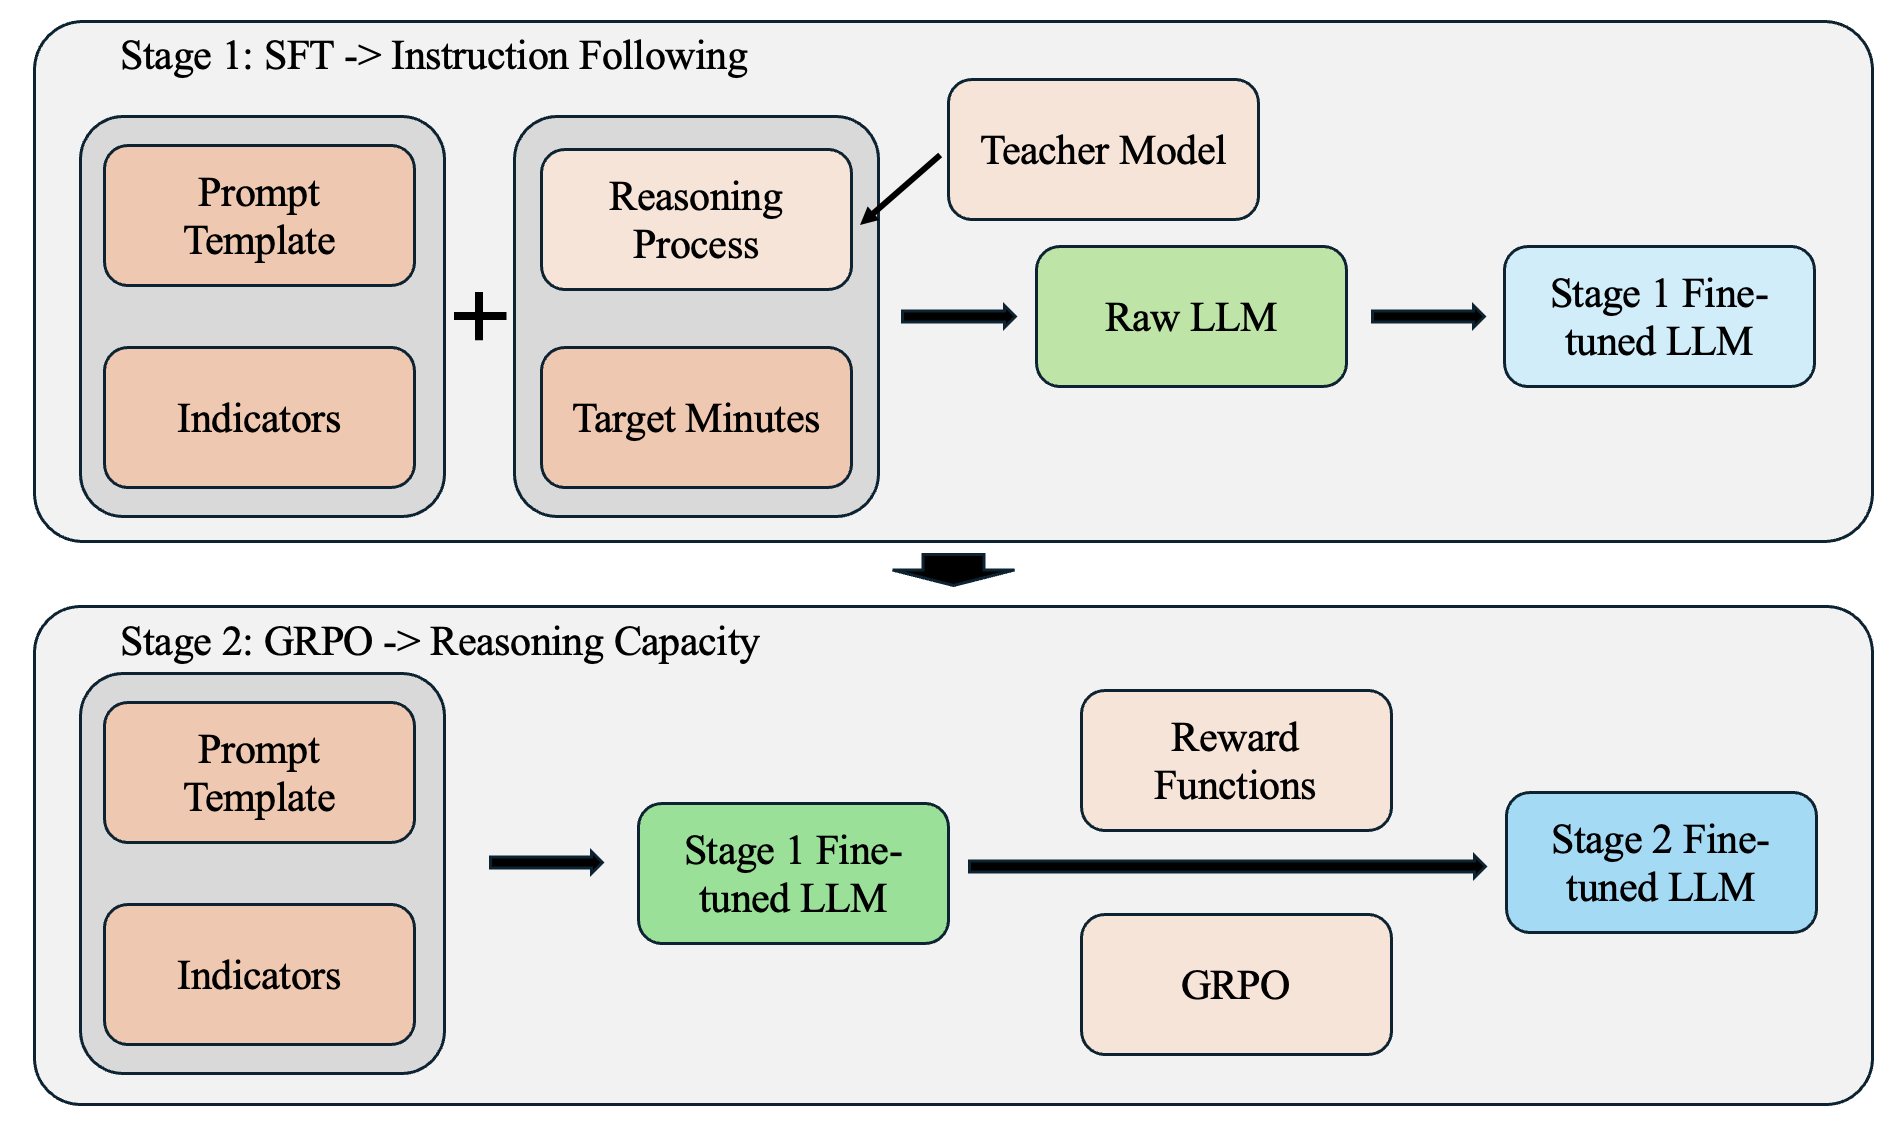
\includegraphics[width=\textwidth]{Chapter2/Chapter2Figs/training_process.png}
    % \caption{Overview of 2-Stage Training Process}
    % [Codex 修改版] 2026-02-26
    \caption{Overview of Two-step Training Process}
    \label{fig:ch2:training_process}
\end{figure}




% In \textit{Stage 1}, we employ a two-step training strategy that combines Supervised Fine-Tuning (SFT) and Group Relative Policy Optimization (GRPO). In \textit{Stage 2}, we focus on synthetic FOMC Minutes generation, the model must reformat analytical content into the formal structure and tone of the actual Minutes. Therefore, SFT is employed for this task. 

% In contrast, for FFR prediction, where deeper analytical reasoning and decision-making are required, we apply GRPO to further strengthen the model’s policy inference capabilities.






\subsection*{Model Input}
% [CH2-041][Original Start]
% To start with, we reformat our dataset into the specific templates for our SFT and GRPO.
% [CH2-041][Original End]
We first reformat the dataset into task-specific templates for SFT and GRPO.

% [CH2-042][Original Start]
% For SFT, each input consists of three parts (denoted as $input^{SFT}_i = (q_i, o^{SFT}_i)$, $o^{SFT}_i = (c_i, a_i)$): Question ($q_i$), Reasoning ($c_i$), and Answer ($a_i$). Firstly, the reasoning process and the finally answer will be combined as the model's target output. Then, the input will be reformatted into a Q\&A pair. During the SFT, the model will generate a output ($o_i^* = (c^*_i, a^*_i)$) based on the given question ($q_i$). The target of SFT to minimize the loss ($\mathcal{L}^{SFT}$) between the $(c^*_i, a^*_i)$ and $(c_i, a_i)$.
% [CH2-042][Original End]
For SFT, each sample is represented as $input_i^{SFT}=(q_i,o_i^{SFT})$, where $o_i^{SFT}=(c_i,a_i)$ contains a reasoning trace ($c_i$) and a final answer ($a_i$). The model predicts $o_i^*=(c_i^*,a_i^*)$ from question $q_i$, and training minimizes supervised loss $\mathcal{L}^{SFT}$ between predicted and target outputs.


% [CH2-043][Original Start]
% For RL training, we only use Questions ($input^{RL}_i = q_i$) as our input. The model will generate the output ($o^{RL}_i = (c_i, a_i)$) by optimizing a given reward function ($\mathcal{R}$)
% [CH2-043][Original End]
For RL training, we use only the question as input ($input_i^{RL}=q_i$). The model generates $o_i^{RL}=(c_i,a_i)$ and is updated to maximize the reward function $\mathcal{R}$.



% [CH2-044][Original Start]
% Moreover, each LLM has its own required format for input texts, as the tokenizer encodes input text into a sequence of tokens. Special labels are used specifically to distinguish the sections: the ``\texttt{System Prompt}'', ``\texttt{User Prompt}'', and ``\texttt{Assistant Response}''. Table. \ref{tab:ch2:input_template_for_llama3} presents the labels used by LLAMA3, where ``\prompttag{start\_header\_id}'' and ``\prompttag{end\_header\_id}'' wrap around the role labels indicating the message type. The label ``\prompttag{begin\_of\_text}'' signals the start of the conversation, while ``\prompttag{end\_id}'' denotes its end.
% [CH2-044][Original End]
Each LLM requires a model-specific message format because tokenizers encode role boundaries differently. We therefore use explicit role tags for system, user, and assistant messages. Table~\ref{tab:ch2:input_template_for_llama3} shows the LLaMA 3 template, where ``\prompttag{start\_header\_id}'' and ``\prompttag{end\_header\_id}'' wrap role labels, ``\prompttag{begin\_of\_text}'' starts the sequence, and ``\prompttag{end\_id}'' terminates it.


\begin{table}[h]
    \centering
    \footnotesize
    \begin{tabular}{p{0.98\textwidth}}
    \toprule
    \textbf{Special Labels for LLaMA 3:} \\
    \midrule
    \prompttag{begin\_of\_text} \\
    \prompttag{start\_header\_id} \textcolor{red}{system}\prompttag{end\_header\_id} \\
    \texttt{... System Prompts ...} \\
    \prompttag{start\_header\_id} \textcolor{red}{user}\prompttag{end\_header\_id} \\
    \texttt{... User Prompts ...} \\
    \prompttag{start\_header\_id} \textcolor{red}{assistant}\prompttag{end\_header\_id} \\
    \texttt{... Assistant Response ...} \\
    \prompttag{end\_id} \\
    \bottomrule
    \end{tabular}
    \caption{Input Template for LLAMA3}
    \label{tab:ch2:input_template_for_llama3}
\end{table}



\subsection*{Incorporate Reasoning Process}

% [CH2-045][Original Start]
% Compared with traditional LLMs, fine-tuning Reasoning Large Language Models (RLLMs) requires explicitly incorporating the reasoning process into the target answers. Recent literature commonly uses special markers, such as ``\texttt{<think>}'' and ``\texttt{</think>}'', to denote the intermediate reasoning trajectory, and ``\texttt{<answer>}'' and ``\texttt{</answer>}'' to clearly indicate the final response. Therefore, our target output ($o_i$) comprises a reasoning trajectory ($c_i$) and a final response ($a_i$), structured as follows:
% [CH2-045][Original End]
Relative to standard chat fine-tuning, reasoning-oriented training requires explicit supervision of intermediate reasoning and final answers. We use ``\texttt{<think>}...\texttt{</think>}'' for reasoning traces and ``\texttt{<answer>}...\texttt{</answer>}'' for final outputs. The target format is:



\begin{equation*}
    o_i = \text{\texttt{<think>}}c_i\text{\texttt{</think>}}\text{\texttt{<answer>}}a_i\text{\texttt{</answer>}}
\end{equation*}


% [CH2-046][Original Start]
% Additionally, to reinforce adherence to this structured format, we employed a dedicated \textbf{System Prompt}, illustrated in Table~\ref{tab:ch2:system_prompt}. The \textbf{System Prompt} typically contains instructions or guidelines that establish a clear framework for guiding the mol to generate relevant and structured responses. For instance, Claude Opus 4 (\cite{claude42025}) utilizes system prompts to convey essential metadata, such as the current date, knowledge cutoff, model identification, and user guidance.
% [CH2-046][Original End]
To improve format compliance, we add a dedicated \textbf{system prompt} (Table~\ref{tab:ch2:system_prompt}) that enforces output tags and response structure.

\begin{table}[h]
    \centering
    \footnotesize
    \begin{tabular}{p{0.98\textwidth}}
    \toprule
    \textbf{System Prompt:} \\
    \midrule
      You are a helpful AI Assistant, designed to provide well-reasoned and detailed responses. \\
  You FIRST think about the reasoning process as an internal monologue and then provide the user with the answer.  \\
  The reasoning process \textbf{MUST BE} enclosed within \texttt{<think>} and \texttt{</think>} tags. The answer MUST BE enclosed within \texttt{<answer>} and \texttt{</answer>} tags. \\
    \bottomrule
    \end{tabular}
    \caption{System Prompt for LLAMA3}
    \label{tab:ch2:system_prompt}
\end{table}




% System Prompts
% See updates to the core system prompts on Claude.ai and the Claude iOS and Android apps.

% Claude's web interface (Claude.ai) and mobile apps use a system prompt to provide up-to-date information, such as the current date, to Claude at the start of every conversation. We also use the system prompt to encourage certain behaviors, such as always providing code snippets in Markdown. We periodically update this prompt as we continue to improve Claude’s responses. These system prompt updates do not apply to the Anthropic API. Updates between versions are bolded.


% These prompts act as a framework, setting the stage for the AI to operate within specific parameters and generate responses that are coherent, relevant, and aligned with the desired outcome. 
% system prompts are a set of instructions, guidelines, and contextual information provided to AI models before they engage with user queries. 





%  o1 thinks before it answers—it can produce a long chain of thought before responding
% to the user.

% We trained these models to spend more time thinking through problems before they respond, much like a person would. Through training, they learn to refine their thinking process, try different strategies, and recognize their mistakes

% The o1 model series is trained with large-scale reinforcement learning to reason using chain-of-thought.

% This complexity is further compounded when reasoning over ambiguous, noisy, or incomplete information.



\subsection*{Supervised Fine-Tuning}
% [CH2-047][Original Start]
% In this section, we explain the input for the Supervised Fine-Tuning (SFT). The SFT process aims at enhancing model's ability in financial analysis. The model will learn to generate a logical reasoning process and draw a similar conclusion as the required output. 4 main steps involves in fine-tuning. Firstly, we need to prepare training dataset. Q\&A pairs are required for SFT. Then, we need to design system and user prompts. Well-structured prompts can help the model generate logical outputs. After that, we employ quantization method, such as LoRA, for partial-parameter FT to reduce the computational costs. Finally, the the loss will be calculated by comparing the target response with the output generated by the model. The process will keep iterating until the convergence of the loss function. Fig. \ref{fig:ch2:ft_detail} illustrates the fine-tuning process:
% [CH2-047][Original End]
This subsection describes SFT inputs and optimization flow. SFT is used to improve domain-specific analytical generation by supervising both reasoning traces and final answers. The workflow includes four steps: preparing Q\&A training data, defining system and user prompts, applying parameter-efficient fine-tuning, and minimizing supervised loss until convergence. Figure~\ref{fig:ch2:ft_detail} illustrates the process.

\begin{figure}
    \begin{center}
        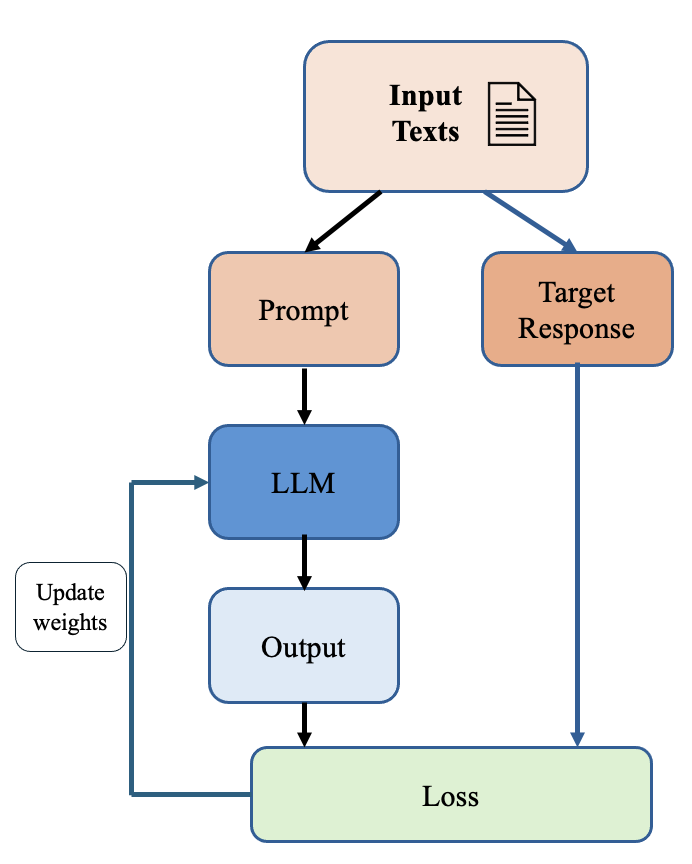
\includegraphics[width=0.3\textwidth]{Chapter2/Chapter2Figs/ft_detail.png}
      \end{center}
      \caption{Fine-Tune Process Flow Chart}
      \label{fig:ch2:ft_detail}
\end{figure}


% [CH2-048][Original Start]
% For example, we want to conduct an analysis on the current inflation rate. We use Personal Consumption Expenditures (PCE) Index as the key indicator. We construct the input prompt ($q_i$) as (Table \ref{tab:ch2:sft_user_prompt_example}):
% [CH2-048][Original End]
As an example, consider inflation analysis using the Personal Consumption Expenditures (PCE) indicator set. The corresponding input prompt $q_i$ is shown in Table~\ref{tab:ch2:sft_user_prompt_example}.

\begin{table}[h]
    \centering
    \footnotesize
    \begin{tabular}{p{0.98\textwidth}}
    \toprule
    \textbf{User Prompt ($q_i$):} \\
    \midrule
    You are an economist preparing briefing notes for the Federal Open Market Committee (FOMC) meeting on \textbf{2023-07-26 00:00:00}. Your task is to analyze recent trends in \textbf{Personal Consumption Expenditures (PCE)} and related indicators, writing in the tone and style of the \textbf{Developments in Financial Markets and Open Market Operations} section of the FOMC minutes. \\
    
    Use neutral, data-driven, and measured language throughout your response. \\
    
    Your analysis \textbf{must} be based on the following indicators: 
    \begin{itemize}
        \item \texttt{Personal Consumption Expenditures Index (Index 2017=100, Seasonally Adjusted).csv}
        \item \texttt{Personal consumption expenditures by major function (Index numbers, 2017=100; quarters and months are seasonally adjusted).xlsx}
        \item \texttt{Personal consumption expenditures by major function (Millions of dollars; quarters and months are seasonally adjusted at annual rates).xlsx}
    \end{itemize}

    Using the accompanying data tables from the past two years provided below: \\

    \vspace{0.5em}
    \textbf{Indicators: Personal Consumption Expenditures (PCE)} \\
    \texttt{Personal Consumption Expenditures Index (Index 2017=100, Seasonally Adjusted).csv} \\
    
    \begin{tabular}{|l|l|}
    \hline
    \texttt{observation\_date} & \texttt{PCEPI} \\
    \hline
    2021-08-01 & 109.72 \\
    2021-09-01 & 110.047 \\
    \vdots & \vdots \\
    2023-06-01 & 120.435 \\
    2023-07-01 & 120.598 \\
    \hline
    \end{tabular} \\

    \vspace{0.5em}
    Keep your response focused, analytically rigorous, and under 4096 tokens. \\
    \bottomrule
    \end{tabular}
    \caption{SFT User Prompt Example}
    \label{tab:ch2:sft_user_prompt_example}
\end{table}



% [CH2-049][Original Start]
% The target output consists of the Reasoning process ($c_i$) and Answer ($a_i$), we firstly wrapped the Reasoning process using \textbf{\texttt{\textless think\textgreater ... \textless /think\textgreater}} and the Answer using \textbf{\texttt{\textless answer\textgreater ... \textless /answer\textgreater}}. Then we combined these two parts as our target output ($o_i = (c_i, a_i)$)(Table. \ref{tab:ch2:sft_target_output_example}):
% [CH2-049][Original End]
The target output combines reasoning ($c_i$) and answer ($a_i$): reasoning is wrapped in \texttt{<think>...</think>} and the final answer in \texttt{<answer>...</answer>}. The combined target $o_i=(c_i,a_i)$ is illustrated in Table~\ref{tab:ch2:sft_target_output_example}.


\begin{table}[h]
    \centering
    \footnotesize
    \begin{tabular}{p{0.98\textwidth}}
    \toprule
    \textbf{Target Output ($o_i = (c_i, a_i)$):} \\
    \midrule
    \textbf{\textless think\textgreater} Okay, I need to prepare a briefing note for the FOMC meeting based on the provided data. The user wants an analysis of recent trends in PCE and related indicators, structured like the \textquotedblleft Developments in Financial Markets and Open Market Operations\textquotedblright{} section from the FOMC minutes. The tone needs to be neutral, data-driven, and measured. Let's start by looking at the data given. \\

    First, the Personal Consumption Expenditures Index (PCEPI) shows a steady increase from 109.72 in August 2021 to 120.598 in July 2023. The monthly growth rates have slowed in recent months. \\

    ... ... \\

    Finally, tie this into the broader economic context, like the potential for a delayed recession and inflation moving towards 2\% by 2025 as per the survey mentioned in the example. \\

    Make sure the language is neutral, avoid speculation, and stick strictly to the data provided. Use terms like ``moderated'', ``deceleration'', ``partially offset'', and ``notable contributions''. Structure the analysis into sections: overall PCE trends, sectoral breakdown, and implications for inflation outlook. Avoid mentioning any data not provided, and ensure all points are backed by the numbers given. \textbf{\textless /think\textgreater} \\[1ex]

    \textbf{\textless answer\textgreater} \textbf{Developments in Personal Consumption Expenditures and Implications for Inflation} \\

    Recent data through July 2023 indicate sustained growth in personal consumption expenditures (PCE), albeit with moderating momentum in key categories. The PCE Price Index (PCEPI) rose to 120.60 in July 2023, reflecting a 3.6\% year-over-year increase, down from the 5.9\% pace observed in July 2022. Monthly gains have decelerated notably, with the index advancing at an average rate of 0.16\% over the three months ending in July. \\

    ... ... \\

    While consumption growth remains positive, real outlays are being constrained by tighter financial conditions and moderating excess savings. This dynamic supports a baseline of below-trend GDP growth with incremental labor market rebalancing, reducing the risk of entrenched inflation expectations. However, the resilience in wage-sensitive services categories warrants continued vigilance regarding price-setting behavior. \textbf{\textless /answer\textgreater} \\
    \bottomrule
    \end{tabular}
    \caption{SFT Target Output Example}
    \label{tab:ch2:sft_target_output_example}
\end{table}


% [CH2-050][Original Start]
% The refinement of the model through retraining employs stochastic gradient descent (SGD) to iteratively adjust the model parameters ($\theta$) based on the \textit{loss function}. In partial fine-tuning (Partial FT), the update process selectively modifies certain layers while leaving others unchanged by zeroing out their gradients. This targeted approach enables the model to adapt to new tasks while preserving the knowledge learned during pre-training.
% [CH2-050][Original End]
Model refinement is performed with stochastic gradient descent (SGD), updating parameters $\theta$ according to the training loss. Under partial fine-tuning, only selected layers are trainable, while frozen layers keep pre-trained knowledge intact.

% [CH2-051][Original Start]
% During SFT training, the \textit{loss} is calculated as the discrepancy between the model's generated responses ($\bm{o^*} \in R^{m\times n}$) and the target responses ($\bm{o}^{SFT} \in R^{m \times n}$). This discrepancy is quantified by the multi-class Cross Entropy Loss ($\mathcal{L}^{CE}$):
% [CH2-051][Original End]
During SFT, the objective is the discrepancy between generated responses ($\bm{o^*}\in\mathbb{R}^{m\times n}$) and targets ($\bm{o}^{SFT}\in\mathbb{R}^{m\times n}$), measured by multi-class cross-entropy loss $\mathcal{L}^{CE}$:


\begin{equation*}
  \mathcal{L}^{CE} = -\frac{1}{n}\sum_{i=1}^{n} o^{SFT}_{k, i}\log  o^*_i(y_i|x_1, x_2, \dots,x_m, y_1, y_2, \dots, y_{i-1}; \theta)
\end{equation*}



% [CH2-052][Original Start]
% where $o_{k,i} = [o_1, o_2, \cdots, o_k, \cdots, o_m]$ is a unit vector with $o_k = 1$ (also known as one-hot encoded vector), which represents the target token, $o^*_i(\cdot)$ denotes the probabilities for the predicted token given the input tokens $\bm{x}$ and previously generated words $\bm{y}$, which are always smaller than 1. Here, the $n$ is the total number of words in the generated response sequence. The Cross Entropy Loss ($\mathcal{L}_{CE}$) represents sum of the negative log probabilities that the model assigns to the target tokens. The correct probabilities will occur when $o_{k,i}=o^*_i(\cdot) = 1$ and $\mathcal{L}^{CE}=0$. Therefore, the objective of the SFT is to minimize $\mathcal{L}^{CE}$ by updating the model's weights $\theta$.
% [CH2-052][Original End]
where $o_{k,i}$ is a one-hot vector identifying the target token at position $i$, and $o_i^*(\cdot)$ is the model-assigned probability for each candidate token given inputs $\bm{x}$ and previously generated tokens $\bm{y}_{<i}$. The sequence length is $n$. Cross-entropy sums negative log probabilities assigned to target tokens; lower values indicate better alignment with supervision. SFT therefore minimizes $\mathcal{L}^{CE}$ by updating $\theta$.





\subsection*{Reinforcement Learning}\label{ch2:sec:model_train:rl}
% Reinforcement Learning (RL) requires the model to update the parameters ($\theta$) by optimizing the feedback. Here, we employed Group Relative Policy Optimization (GRPO) in this stage.

% [CH2-053][Original Start]
% Reinforcement Learning (RL) requires the model to update parameters ($\theta$) by optimizing feedback. Different from the Supervised Fine-Tuning, the target of the Reinforcement Learning is to maximize the feedback by changing the way of producing the output. As the same analysis can be constructed in different ways, RL serves as a significantly in booting the model's reasoning ability, such as the ChatGPT o1 (\cite{jaech2024openai}) and the Deepseek-R1 (\cite{guo2025deepseek}) for general purpose, the Fin-R1 \cite{liu2025fin} and the Fino1 \cite{qian2025fino1} in finance domain.
% [CH2-053][Original End]
Reinforcement learning (RL) updates parameters $\theta$ by maximizing feedback signals rather than matching fixed token-level targets. This is useful in analytical tasks where multiple valid response paths exist. Recent reasoning models (e.g., ChatGPT o1, DeepSeek-R1, Fin-R1, Fino1) illustrate the value of RL-style optimization for reasoning-heavy outputs (\cite{jaech2024openai}; \cite{guo2025deepseek}; \cite{liu2025fin}; \cite{qian2025fino1}).

More specifically, in this stage, we employed Group Relative Policy Optimization (GRPO, \cite{shao2024deepseekmath}).

% [CH2-054][Original Start]
% GRPO is an on-policy reinforcement learning algorithm derived from the Proximal Policy Optimization algorithm (PPO, \cite{schulman2017proximal}). PPO is a policy-gradient-based reinforcement learning technique designed for stable optimization. It requires the model to maximize a reward signal ($A_t$), provided by a reward function, by generating outputs from the current policy model ($\pi_{\theta}$). Unlike Supervised Fine-Tuning, RL does not rely on predefined target outputs. Instead, it uses a scoring function to evaluate model outputs. This score, known as the reward, serves as feedback for model training. The goal of training is to maximize an objective function ($\mathcal{J}(\theta)$) defined in terms of the reward. Consequently, only the question ($q_i$) is included in the training input ($input^{RL}_i$).
% [CH2-054][Original End]
GRPO is an on-policy RL algorithm derived from Proximal Policy Optimization (PPO; \cite{schulman2017proximal}). In this framework, the policy $\pi_\theta$ is optimized to maximize a reward-driven objective $\mathcal{J}(\theta)$. Unlike SFT, RL training does not require reference targets; the model is scored by a reward function based on generated outputs. Therefore, only the question $q_i$ is required as training input.


% [CH2-055][Original Start]
% Additionally, PPO employs a clipping function ($CLIP(\cdot)$) to scale the reward in the objective function, enhancing training stability. The model parameters ($\theta$) are updated using stochastic gradient descent (SGD) until the objective function is maximized. The objective function ($\mathcal{J}^{\text{PPO}}$) is given by:
% [CH2-055][Original End]
PPO applies a clipping operator $CLIP(\cdot)$ for stable policy updates. Parameters $\theta$ are optimized with SGD to maximize the PPO objective:




\begin{footnotesize}
    \begin{equation}
        \begin{split}
            \mathcal{J}^{\text{PPO}}(\theta) =
             &\mathbb{E}_{q\sim P(Q), o\sim\pi_{\theta_{\text{old}}}(O|q)}\frac{1}{|o|}\sum_{t=1}^{|o|}\Bigg[\min\Bigg\{ \\
             &\frac{\pi_{\theta}(o_t | q, o_{<t})}{\pi_{\theta_{\text{old}}}(o_t | q, o_{<t})} A_t(r_t, v_t), \text{CLIP}\left(\frac{\pi_{\theta}(o_t | q, o_{<t})}{\pi_{\theta_{\text{old}}}(o_t | q, o_{<t})}, 1 - \epsilon, 1+\epsilon\right)A_t(r_t, v_t)\Bigg\}\Bigg]
        \end{split}
    \end{equation}
\end{footnotesize}



where:

\begin{equation*}
r_t = r_\phi(q, o_{\leq t}) - \beta \log\frac{\pi_{\theta}(o_t | q, o_{<t})}{\pi_{\text{ref}}(o_t | q, o_{<t})}
\end{equation*}

\begin{equation*}
v_t = V_t(o_t | q, o_{<t})
\end{equation*}

Here, $\pi_{\theta}$ represents our trainable \textit{policy model}. $r_t$ is the KL-divergence adjusted reward, where $r_\phi$ is the reward from the \textit{reward model}. $\pi_{\text{ref}}$ is the \textit{reference model}, initialized as a copy of the original policy model. $V_t(\cdot)$ denotes a trainable \textit{value model} used to estimate expected rewards, aiding the policy in exceeding baseline expectations. $A_t$ is the advantage function, providing final feedback to the model, typically calculated using Generalized Advantage Estimation (GAE). $\beta$ is the penalty coefficient for KL divergence, while $\epsilon$ controls the extent of clipping. Both $\beta$ and $\epsilon$ are hyperparameters crucial for maintaining training stability.

However, the training cost for the PPO is significantly higher than the Supervised Fine-Tuning. In PPO, four models, the policy model, the reference model, the reward model, and the value model, need to be loaded. Two models, the policy model and the value model, are being trained at the same time. To address the issue, we employed the Group Relative Policy Optimization (GRPO), which removed the value model by calculating the relative average reward from multiple sampled outputs as the advantage. The objective function for GRPO ($\mathcal{J}^{\text{GRPO}}$) is given by:




\begin{footnotesize}
    \begin{equation}
        \begin{split}
            \mathcal{J}^{\text{GRPO}}(\theta) 
            &= \mathbb{E}_{q \sim P(Q), \{o\}^G_{i=1} \sim \pi_{\theta_{\text{old}}}(O \mid q)} \Bigg[ \frac{1}{G} \sum_{i=1}^{G} \frac{1}{|o_i|} \sum_{t=1}^{|o_i|} \Bigg\{ \nonumber \\
            &\quad \min \Bigg( 
                \frac{ \pi_{\theta}(o_{i,t} \mid q, o_{i,<t}) }{ \pi_{\theta_{\text{old}}}(o_{i,t} \mid q, o_{i,<t}) } \hat{A}_{i,t}(r_{i,t}), \;
                \text{CLIP}\left( \frac{ \pi_{\theta}(o_{i,t} \mid q, o_{i,<t}) }{ \pi_{\theta_{\text{old}}}(o_{i,t} \mid q, o_{i,<t}) }, 1 - \epsilon, 1 + \epsilon \right) \hat{A}_{i,t}(r_{i,t}) 
            \Bigg) \nonumber \\
            &\quad - \beta \, \mathbb{D}_{\text{KL}}\left[ \pi_{\theta} \,\|\, \pi_{\text{ref}} \right] 
            \Bigg\} \Bigg]
        \end{split}
    \end{equation}
\end{footnotesize}




where:

\begin{equation*}
    \hat{A}_{i,t}(r_{i, t}) = \frac{r_{i, t} - \text{mean}(\mathbf{r}_t)}{\text{std}(\mathbf{r}_t)}
\end{equation*}

\begin{equation*}
    \mathbb{D}_{KL}[\pi_{\theta} || \pi_{ref}] = \frac{\pi_{\text{ref}}(o_{i, t} | q, o_{i, <t})}{\pi_{\theta}(o_{i, t} | q, o_{i, <t})} - \log \frac{\pi_{\text{ref}}(o_{i, t} | q, o_{i, <t})}{\pi_{\theta}(o_{i, t} | q, o_{i, <t})} - 1
\end{equation*}


% [CH2-056][Original Start]
% Here, $G$ is the size of the sampled outputs for each iteration $t$. $r_{i,t}$ is reward for output $i$ at iteration $t$. Instead of training a \textit{value model} in calculating the expected rewards, the GRPO uses the sum of the normalized rewards from a sample outputs of size $G$ as the advantage function $\hat{A}_{i,t}$. Additionally, the KL divergence penalty is added directly to the objective function to reduce the calculation cost in the advantage function. As a result, the training cost has been significantly reduced by applying the GRPO.
% [CH2-056][Original End]
Here, $G$ denotes the number of sampled outputs per iteration and $r_{i,t}$ is the reward for output $i$ at step $t$. GRPO avoids a separately trained value model by computing relative advantages from group-normalized rewards. A KL penalty is included directly in the objective to constrain policy drift from the reference model. This design lowers training cost while preserving optimization stability.

% [CH2-057][Original Start]
% Finally, to implement the GRPO, we use the same \textit{User Prompt ($q_i$)} (see Table~\ref{tab:ch2:sft_user_prompt_example}) as the SFT stage as our input. Then, we adopt the idea of ``LLM as Judge'' by using another powerful model as our reward model to score the output from our policy model.
% [CH2-057][Original End]
In implementation, GRPO uses the same user prompt template as SFT (Table~\ref{tab:ch2:sft_user_prompt_example}). Rewards are assigned with an LLM-as-Judge setup, where a stronger evaluator model scores policy outputs.

% [Codex 修改版] 2026-04-17: 明确 teacher / judge / legacy service 的实际实现位置，避免正文与脚本说明混淆。
\subsection*{External Models and Implementation Roles}

\begin{table}[htbp]
    \centering
    \footnotesize
    \begin{tabular}{p{0.2\textwidth} p{0.24\textwidth} p{0.5\textwidth}}
    \toprule
    \textbf{Role} & \textbf{Model / Script} & \textbf{Use in This Chapter} \\
    \midrule
    Teacher model & \texttt{DeepSeek-R1} & Generates distilled reasoning traces during dataset construction for both analysis and Minutes-style alignment tasks. \\
    Reward judge for analysis GRPO & \texttt{gemma3:12b} in \texttt{src/open\_r1/trainer/rewards/reward\_funcs/online\_reward.py} & Scores format compliance, answer quality, and reasoning consistency for Checkpoint-2 via a local HTTP endpoint (\texttt{http://localhost:11432/api/chat/}). \\
    Legacy / alternative serving script & \texttt{start\_vllm.sh} & Starts a vLLM OpenAI-compatible server for the policy model on port 8000. This script is retained for serving and experimentation, but it is not the active reward-judge path used by the archived analysis GRPO implementation. \\
    \bottomrule
\end{tabular}
    \caption{External Models and Service Roles in the Archived Training Pipeline}
    \label{tab:ch2:external_model_roles}
\end{table}

% [Codex 修改版] 2026-04-17: 说明 teacher / judge 已可追溯，但版本号和硬件元数据并未在当前归档中完整保存。
Table~\ref{tab:ch2:external_model_roles} resolves the teacher/judge role confusion for the archived runs reported in this chapter. At the same time, the repository does \textit{not} preserve a complete machine-readable record of external model version strings, serving dates, or hardware inventory. We therefore report only the components that can be recovered directly from the archived code and artifacts.



\subsection*{Reward Function Design}\label{ch2:sec:mode_training:reward_function}
% 

% [CH2-058][Original Start]
% Inspired by existing literature, we adopt a two-aspect reward framework comprising a format reward and an accuracy reward. For each stage of GRPO training, we design multiple reward functions to guide the model’s behavior in alignment with specific task objectives.
% [CH2-058][Original End]
% [CH2-112][Original Start]
% Following prior work, we use a multi-component reward design. The core components are format compliance, analytical quality, and reasoning coherence.
% [CH2-112][Original End]
Following prior work, we design three complementary reward components for analytical GRPO: format compliance, answer-level analytical quality, and reasoning coherence. In the canonical Checkpoint-2 configuration, all three are active. The format reward enforces the tagged output contract, while the answer and reasoning rewards are provided by an LLM-as-Judge service. Their weights are fixed at $0.2$, $0.4$, and $0.4$, respectively.

% [CH2-059][Original Start]
% In the RL training stage, the focus is on enhancing the model’s analytical ability. Unlike mathematical reasoning tasks, economic and financial analyses do not always yield a single ``correct'' answer. To address this, we employ the ``LLM-as-Judge framework'' (\cite{zheng2024judging}) to evaluate both the reasoning process and the final analysis. Several key criteria are used for this evaluation, with the reward model assessing the output and assigning a score accordingly. Specifically, we design the following reward components: the \textit{Format Reward} ($\mathcal{R}_{fmt}(o_i)$), the \textit{Accuracy Reward} ($\mathcal{R}_{acc}(o_i)$), and the \textit{Reasoning Reward} ($\mathcal{R}_{reason}(o_i)$).
% [CH2-059][Original End]
% [CH2-113][Original Start]
% RL training targets analytical quality. Because macro-financial analysis does not have a unique ground-truth answer, we evaluate outputs with an LLM-as-Judge framework (\cite{zheng2024judging}). We use three reward components: \textit{Format Reward} $\mathcal{R}_{fmt}(o_i)$, \textit{Accuracy Reward} $\mathcal{R}_{acc}(o_i)$, and \textit{Reasoning Reward} $\mathcal{R}_{reason}(o_i)$.
% [CH2-113][Original End]
RL training targets analytical quality. Because macro-financial analysis does not have a unique ground-truth answer, we evaluate outputs with an LLM-as-Judge framework (\cite{zheng2024judging}). For exposition, we describe three components: \textit{Format Reward} $\mathcal{R}_{fmt}(o_i)$, \textit{Answer Reward} $\mathcal{R}_{\text{answer}}(o_i)$, and \textit{Reasoning Reward} $\mathcal{R}_{\text{reason}}(o_i)$. In the decision-specific GRPO branch, the active rewards differ: the archived run uses \textit{rate accuracy} and \textit{rate format}, each with unit weight.


% In Stage 2, the primary objective shifts to improving prediction accuracy, and unlike Stage 1, this task has a clearly defined correct answer. As a result, the emphasis moves toward output correctness. Accordingly, we introduce the \textit{Vote Accuracy Reward} ($\mathcal{R}_{vote\_acc}(o_i)$) and the \textit{Vote Format Reward} ($\mathcal{R}_{vote\_fmt}(o_i)$), both designed to reinforce precision and consistency in generating accurate policy decisions.

% [CH2-114][Original Start]
% Finally, the \textit{Total Reward} is computed as the sum of the individual reward components. The model updates its parameters based on the \textit{Total Reward} obtained from the most recent generation.
% [CH2-114][Original End]
For any given run, the \textit{Total Reward} is computed from the subset of reward functions activated in the corresponding configuration. Consequently, the total reward shown for Checkpoint-2 should be interpreted as the weighted combination of format, answer, and reasoning rewards, whereas the decision-specific Checkpoint-4 branch uses the sum of rate-accuracy and rate-format rewards.

% [Codex 修改版] 2026-04-17: 将当前章实际使用的 reward 汇总写成明确公式，避免正文与实现不一致。
\begin{equation}\label{eq:ch2:analysis_total_reward}
    \mathcal{R}^{\text{Checkpoint-2}}_{\text{total}}(o_i)
    = 0.2 \cdot \mathcal{R}_{\text{fmt}}(o_i)
    + 0.4 \cdot \mathcal{R}_{\text{answer}}(o_i)
    + 0.4 \cdot \mathcal{R}_{\text{reason}}(o_i)
\end{equation}

\begin{equation}\label{eq:ch2:decision_total_reward}
    \mathcal{R}^{\text{Checkpoint-4}}_{\text{total}}(o_i)
    = \mathcal{R}_{\text{rate-acc}}(o_i)
    + \mathcal{R}_{\text{rate-fmt}}(o_i)
\end{equation}


\subsubsection*{Format Reward}
% [CH2-060][Original Start]
% To ensure the reasoning process, we require the model to generate the output in the specific format. The reasoning process should be wrapped with \textbf{\texttt{\textless think\textgreater ... \textless /think\textgreater}} and the answer should be wrapped with \textbf{\texttt{\textless answer\textgreater ... \textless /answer\textgreater}}. Therefore, we designed a format reward function ($\mathcal{R}_{fmt}(\cdot)$) checking the output. A correct format will be scored as 1 while the wrong format will be marked as 0:
% [CH2-060][Original End]
To enforce output structure, reasoning must appear in \texttt{<think>...</think>} and the final response in \texttt{<answer>...</answer>}. The format reward is binary:


\begin{equation}\label{eq:ch2:format_reward}
    \mathcal{R}_{\text{fmt}}(o_i) = 
    \begin{cases}
        1, & \text{if the format is correct} \\
        0, & \text{if the format is wrong}
    \end{cases}
\end{equation}




\subsubsection*{Answer Reward}

% [CH2-061][Original Start]
% Unlike previous studies that trained their models on publicly available datasets, such as FinQA (\cite{chen2021finqa}), our training target is to generate comprehensive and logical economic and financial analyses. Since there is no fixed or predefined correct answer for such analyses, we adopt the "LLM as Judge" framework (\cite{zheng2023judging}) for our reward model. Instead of creating a mathematical reward function, we design a prompt that includes the model's generated output. Then, we employ a powerful evaluation model (referred to as the \textit{``reward model''}, denoted by $\mathcal{R}_{acc}(\cdot)$) to score the output based on specific instructions. The resulting score serves as the accuracy reward. However, the reward obtained through this method heavily depends on the quality and clarity of the instructions provided; biased evaluation criteria may lead to biased rewards. To mitigate this issue, we carefully designed seven evaluation dimensions: problem definition, data usage, theoretical support, empirical analysis, analytical depth, policy relevance, and language accuracy. Table~\ref{tab:ch2:llm_as_judge_evaluation} summarizes these seven aspects along with a brief description of each criterion.
% [CH2-061][Original End]
% [CH2-115][Original Start]
% Our objective differs from tasks with fixed answers (e.g., FinQA; \cite{chen2021finqa}). We target comprehensive macro-financial analysis, where multiple valid responses may exist. We therefore use an LLM-as-Judge reward model (\cite{zheng2023judging}) and score outputs with a structured rubric. Because judge-based rewards are prompt-sensitive, we define seven explicit dimensions: problem definition, data usage, theoretical support, empirical methodology, analytical depth, policy relevance, and language quality (Table~\ref{tab:ch2:llm_as_judge_evaluation}).
% [CH2-115][Original End]
Our objective differs from tasks with fixed answers (e.g., FinQA; \cite{chen2021finqa}). We target comprehensive macro-financial analysis, where multiple valid responses may exist. We therefore use an LLM-as-Judge reward model (\cite{zheng2023judging}) and score outputs with a structured rubric. Because this reward primarily evaluates the quality of the final analytical answer, we refer to it hereafter as the \textit{Answer Reward}. The rubric uses seven explicit dimensions: problem definition, data usage, theoretical support, empirical methodology, analytical depth, policy relevance, and language quality (Table~\ref{tab:ch2:llm_as_judge_evaluation}).




\begin{table}[h]
    \centering
    \footnotesize
    \begin{tabular}{p{0.33\textwidth}|p{0.63\textwidth}}
    \toprule
    \textbf{Evaluation Dimension} & \textbf{Evaluation Focus} \\
    \midrule
    \textbf{1. Problem Definition \& Structural Completeness} &
    \parbox[t]{0.65\textwidth}{
        \textbullet\ Is the core research or policy question clearly defined? \newline
        \textbullet\ Is there sufficient background and objective? \newline
        \textbullet\ Is the structure complete (e.g., introduction, method, findings, conclusion)?\newline
        \textbullet\ Is the logical flow coherent from question to conclusion?\newline
} \\
\hline
\textbf{2. Data Usage \& Verifiability} &
\parbox[t]{0.65\textwidth}{
    \textbullet\ Are the data selected from credible sources?\newline
    \textbullet\ Are the data sources clearly cited?\newline
    \textbullet\ Are the data relevant to the argument?\newline
    \textbullet\ Can the analysis be independently verified using the data?\newline
} \\
\hline
\textbf{3. Theoretical Support \& Citations} &
\parbox[t]{0.65\textwidth}{
    \textbullet\ Are appropriate economic or financial theories applied?\newline
    \textbullet\ Are relevant scholarly or institutional sources cited?\newline
    \textbullet\ Are the cited theories or sources correctly interpreted?\newline
} \\
\hline
\textbf{4. Empirical Methodology \& Transparency} &
\parbox[t]{0.65\textwidth}{
    \textbullet\ Are the empirical methods appropriate for the question?\newline
    \textbullet\ Are the methods clearly explained and reproducible?\newline
    \textbullet\ Are assumptions and limitations discussed?\newline
} \\
\hline
\textbf{5. Analytical Depth \& Insight} &
\parbox[t]{0.65\textwidth}{
    \textbullet\ Are key variables correctly identified and analyzed?\newline
    \textbullet\ Does the analysis show meaningful economic or financial insight?\newline
    \textbullet\ Are policy trade-offs or complex relationships discussed?\newline
    \textbullet\ Is there a forward-looking or scenario-based component?\newline
} \\
\hline
\textbf{6. Policy Relevance \& Real-world Significance} &
\parbox[t]{0.65\textwidth}{
    \textbullet\ Are the conclusions tied to real-world policy implications?\newline
    \textbullet\ Does the analysis provide decision-relevant insights?\newline
    \textbullet\ Is the analysis useful for policymakers or market actors?\newline
} \\
\hline
\textbf{7. Clarity \& Language Accuracy} &
\parbox[t]{0.65\textwidth}{
    \textbullet\ Is the language clear, professional, and grammatically correct?\newline
    \textbullet\ Are economic and financial terms used accurately?\newline
    \textbullet\ Is the terminology consistent throughout the analysis?\newline
} \\
\bottomrule
    \end{tabular}
    \caption{Evaluation Criteria for Assessing LLM-Generated Economic/Financial Analyses}
    \label{tab:ch2:llm_as_judge_evaluation}
\end{table}




% ## TODO: add the details about each point


% [CH2-062][Original Start]
% Then, each criterion is scored on a scale from 1 to 5, where 1 indicates "Very Poor" and 5 indicates "Excellent." The \textit{total score}, obtained by summing the individual criterion scores, is then used as the accuracy reward. We employ the prompt shown in Table~\ref{tab:ch2:accuracy_reward_prompt} to format the policy model's output before submitting it to the reward model. Finally, to normalize the reward and balance the influence of different reward functions, the \textit{total score} is divided by 35, resulting in a final accuracy reward ($\mathcal{R}_{\text{acc}}(o_i)$) scaled between 0 and 1.
% [CH2-062][Original End]
% [CH2-116][Original Start]
% Each criterion is scored from 1 to 5 (1 = very poor, 5 = excellent). The summed score is normalized by 35 to produce the final accuracy reward $\mathcal{R}_{\text{acc}}(o_i)\in[0,1]$. Table~\ref{tab:ch2:accuracy_reward_prompt} shows the evaluator prompt.
% [CH2-116][Original End]
Each criterion is scored from 1 to 5 (1 = very poor, 5 = excellent). The summed score is normalized by 35 to produce the final answer reward $\mathcal{R}_{\text{answer}}(o_i)\in[0,1]$. In the canonical analysis GRPO configuration, this component receives weight $0.4$ in the total reward. Table~\ref{tab:ch2:accuracy_reward_prompt} shows the evaluator prompt.


\begin{table}[htbp]
    \centering
    \footnotesize
    \begin{tabular}{p{0.98\textwidth}}
    \toprule
    \textbf{Prompt for Answer Reward ($\mathcal{R}_{\text{answer}}(o_i)$):} \\
    \midrule
    You are an economic and financial policy expert serving as an internal evaluator at the Federal Reserve. You are tasked with \textbf{assessing the analytical quality and fidelity} of a large language model's output based on structured economic/financial data. \\[1ex]

\textbf{Evaluation Criteria (Score each from 1--5):} \\

-- Problem Definition \& Structural Completeness \\
\quad \textit{... description ...} \\

-- Accuracy of Economic Relationships and Logic \\
\quad \textit{... description ...} \\

-- Correct Use of Data and Trends \\
\quad \textit{... description ...} \\[1ex]

\textbf{Scoring Instructions:} \\
- Each category receives an integer score (1--5). \\
-  Justify each score briefly and concisely. \\[1ex]

\textbf{Output Template:} \\
- \textbf{Score}: \texttt{\textbackslash boxed\{\{X\}\}} \\
- \textbf{Justification}: Your explanation in 1--2 sentences. \\[1ex]

\textbf{Input Data:} \\
The model analysis is based on the following indicators: \texttt{\{emphasized\_label\}}. \\

\textbf{\textless Provided Data\textgreater} \\
\texttt{\{provided\_data\}} \\
\textbf{\textless /Provided Data\textgreater} \\[1ex]

\textbf{\textless Model Analysis\textgreater} \\
\texttt{\{model\_analysis\}} \\
\textbf{\textless /Model Analysis\textgreater} \\
\bottomrule
    \end{tabular}
    \caption{Answer-Level Analytical Reward Prompt}
    \label{tab:ch2:accuracy_reward_prompt}
\end{table}

\subsubsection*{Reasoning Reward}

% [CH2-063][Original Start]
% Furthermore, to ensure that the model generates logically coherent responses, we introduced a reasoning reward ($\mathcal{R}_{\text{reason}}(o_i)$) to evaluate the quality of the reasoning trajectory. Similar to our \textit{Accuracy Reward}, we adopted the ``LLM-as-Judge'' framework, using a powerful \textit{reward model} to score the reasoning process. The prompt used for evaluating the reasoning trajectory is presented in Table~\ref{tab:ch2:reasoin_reward_prompt}. The total score for reasoning evaluation is 5, we scaled the score by dividing it by 5 for normalization. Finally, the ``Reasoning Reward ($\mathcal{R}_{\text{reason}}(o_i)$)'' ranges between 0 and 1.
% [CH2-063][Original End]
% [CH2-117][Original Start]
% To enforce logical consistency between reasoning and final answers, we add a reasoning reward $\mathcal{R}_{\text{reason}}(o_i)$. Using the same LLM-as-Judge framework, the evaluator assigns a score from 1 to 5 based on reasoning--answer consistency (Table~\ref{tab:ch2:reasoin_reward_prompt}). We normalize by 5 so that $\mathcal{R}_{\text{reason}}(o_i)\in[0,1]$.
% [CH2-117][Original End]
To enforce logical consistency between reasoning and final answers, we add a reasoning reward $\mathcal{R}_{\text{reason}}(o_i)$. Using the same LLM-as-Judge framework, the evaluator assigns a score from 1 to 5 based on reasoning--answer consistency (Table~\ref{tab:ch2:reasoin_reward_prompt}). We normalize by 5 so that $\mathcal{R}_{\text{reason}}(o_i)\in[0,1]$. In the canonical analysis GRPO configuration, this component receives weight $0.4$.




\begin{table}[htbp]
    \centering
    \footnotesize
    \begin{tabular}{p{0.98\textwidth}}
    \toprule
        \textbf{Prompt for Reasoning Reward ($\mathcal{R}_{\text{reason}}(o_i)$):} \\
    \midrule
    % [CH2-064][Original Start]
    % You are an economic and financial policy expert serving as an internal evaluator at the Federal Reserve. Your task is to assess the **internal logical consistency** between a language model’s reasoning and its final answer. \\
    % [CH2-064][Original End]
    You are an economic and financial policy expert serving as an internal Federal Reserve evaluator. Your task is to assess the **logical consistency** between a model's reasoning and its final answer. \\
    ~\\
    You will be provided with: \\
    - **\textless Model Reasoning\textgreater**: The model’s internal reasoning process.  \\
    - **\textless Model Answer\textgreater**: The model’s final answer or policy recommendation derived from that reasoning. \\

    Your evaluation must be **objective, consistent, and aligned with policy-analysis standards**. \\
    Determine whether the reasoning clearly and sufficiently supports the final answer. \\

    --- \\

    \#\#\# Scoring Criteria (1--5) \\

    1 = Very poor (reasoning contradicts or fails to support the answer). \\
    2 = Weak (reasoning is partial, unclear, or logically weak).  \\
    3 = Acceptable (reasoning and answer are mostly aligned, with minor issues).  \\
    4 = Strong (reasoning supports the answer with good coherence).  \\
    5 = Excellent (reasoning fully supports the answer without logical gaps).\\
    
    --- \\

    \#\#\# Output Instructions:\\

    - Output the score using the format: \texttt{\textbackslash boxed\{\{score\}\}}  \\
    - Then provide a **short paragraph** (1–3 sentences) summarizing the main justification  \\
    - If the reasoning is incoherent, irrelevant, or contradicts the answer, assign a score of **1** \\

    Do **not** explain each criterion separately.  \\
    Only return the final score and the overall justification. \\

    --- \\

    \#\#\# Input \\

    **\textless Model Reasoning\textgreater** \\
    \texttt{\{model\_reasoning\}}\\  
    **\textless /Model Reasoning\textgreater**\\
    ~\\
    **\textless Model Answer\textgreater**  \\
    \texttt{\{model\_analysis\}}  \\
    **\textless /Model Answer\textgreater** \\
    \bottomrule
    \end{tabular}
    \caption{Reasoning Reward Prompt}
    \label{tab:ch2:reasoin_reward_prompt}
\end{table}


% \subsubsection*{Vote Accuracy Reward}
% In Stage 2, we further fine-tuned the model to predict the voting outcomes related to monetary policy decisions in FOMC meetings, specifically concerning the Federal Funds Rate (FFR). To evaluate performance, we parsed the model’s response ($o_i$) and compared it with the ground-truth voting outcome, using this comparison to compute the Vote Accuracy Reward ($\mathcal{R}_{vote\_acc}(o_i)$), as defined in Eq.~(\ref{eq:ch2:vote_acc_reward}).

% \begin{equation}\label{eq:ch2:vote_acc_reward}
%     \mathcal{R}_{vote\_acc}(o_i) = 
%     \begin{cases}
%         1, & \text{if the voting result is correct} \\
%         0, & \text{if the voting result is wrong}
%     \end{cases}
% \end{equation}




% \subsubsection*{Vote Format Reward}

% Furthermore, unlike mathematical calculations, voting results in FOMC contexts may be expressed in various formats, which presents a challenge for consistent evaluation. To address this, we summarized the daily Federal Funds Rate (FFR) changes from January 1, 2000 to May 8, 2025 (see Table~\ref{tab:ch2:ffr_changes}), and constructed a list of standardized potential outcomes (Table~\ref{tab:ch2:vote_choice}). We then instructed the model to select its final vote from this predefined list. Accordingly, the Vote Format Reward (see Eq.~(\ref{eq:ch2:vote_format_reward})) measures whether the model’s predicted decision conforms to one of the allowed options in the list.

% \begin{equation}\label{eq:ch2:vote_format_reward}
%     \mathcal{R}_{vote\_fmt}(o_i) = 
%     \begin{cases}
%         1, & \text{if the voting result is correct} \\
%         0, & \text{if the voting result is wrong}
%     \end{cases}
% \end{equation}



% \begin{table}[htbp]
%     \centering
%     \footnotesize
%     \begin{minipage}[t]{0.48\textwidth}
%         \centering
%         \begin{tabular}{c c}
%             \toprule
%             Rate Change (bps) & Frequency \\
%             \midrule
%             0    & 6,177 \\
%             25   & 31 \\
%             -50  & 15 \\
%             -25  & 12 \\
%             75   & 4 \\
%             50   & 2 \\
%             -75  & 2 \\
%             \bottomrule
%         \end{tabular}
%         \caption{Daily Federal Fund Rate Changes (in BPS) from Jan 1, 2000 to May 9, 2025}
%         \label{tab:ch2:ffr_changes}
%     \end{minipage}
%     \hfill
%     \begin{minipage}[t]{0.48\textwidth}
%         \centering
%         \begin{tabular}{l}
%             \toprule
%             Target Vote Choices \\
%             \midrule
%             Raise by 100 basis points \\
%             Raise by 75 basis points \\
%             Raise by 50 basis points \\
%             Raise by 25 basis points \\
%             No change \\
%             Cut by 25 basis points \\
%             Cut by 50 basis points \\
%             Cut by 75 basis points \\
%             Cut by 100 basis points \\
%             \bottomrule
%         \end{tabular}
%         \caption{Choices for Target Vote}
%         \label{tab:ch2:vote_choice}
%     \end{minipage}
% \end{table}












\subsection*{Technique for Parameter-Efficient Fine-Tuning (PEFT)}

% [CH2-065][Original Start]
% Fine-tuning models to enhance their performance on specific task is a common practice in the NLP. When conducting Full-parameter Fine-Tuning (FT), the entire base model will be updated, leading to enhanced capabilities in generating task-specific text. However, this comes at a significant computational cost.  Full-parameter fine-tune the model requires about 120GB of GPU memory even only for a 8 billion parameters' model. In contrast, Partial-parameter Fine-Tuning (FT) offers more economical alternative, significantly reducing GPU memory requirements by freezing certain layers of the model.
% [CH2-065][Original End]
Fine-tuning for specialized tasks is standard in NLP. Under full-parameter fine-tuning, all base-model weights are updated, which can improve task performance but is computationally expensive. For an 8B-parameter model, full fine-tuning can require roughly 120 GB of GPU memory. Partial fine-tuning reduces this requirement by freezing most layers.


% [CH2-066][Original Start]
% To further optimize memory usage without compromising performance, Parameter-Efficient Fine-Tuning (PEFT) and Quantization techniques, such as LoRA (Low-Rank Adaptation, \cite{hu2021lora}), Quantized Low-Rank Adaptation (QLoRA, \cite{dettmers2024qlora}), and Gated Low-Rank Evolving (GaLoRE, \cite{zhao2024galore}), are employed to significantly reduce memory consumption. PEFT involves fine-tuning only a subset of the model's parameters or introducing additional lightweight trainable layers, rather than updating the full model. Quantization, on the other hand, reduces the precision of model weights to formats such as FP16, FP8, or FP4, thereby lowering the memory footprint. For example, LoRA—widely adopted for its efficiency in the fine-tuning literature—can reduce memory requirements from 120GB to as little as 24GB.
% [CH2-066][Original End]
To reduce memory costs while maintaining performance, we use parameter-efficient fine-tuning (PEFT) with quantization, including LoRA (\cite{hu2021lora}), QLoRA (\cite{dettmers2024qlora}), and related methods such as GaLoRE (\cite{zhao2024galore}). PEFT updates only a small subset of parameters or adds lightweight trainable adapters. Quantization lowers precision (e.g., FP16/FP8/FP4) and further reduces memory usage. In practical settings, LoRA-style adaptation can reduce memory requirements from around 120 GB to roughly 24 GB.


% [CH2-067][Original Start]
% LoRA's mechanism involves introducing additional layers, referred to as Adapters, with a much smaller rank (typically 1 or 2) compared to the pre-trained weight matrices (such as 2048 in the LLaMA3 model). These Adapters are specifically designed for the task at hand and undergo training during the fine-tuning process. Upon completion of training, these adapted layers are merged back into the base model, effectively enhancing its capabilities for the target task while keeping the overall memory footprint minimal. This approach not only facilitates the fine-tuning of large models on resource-constrained environments but also allows for the integration of task-specific knowledge without the need to retrain the entire model from scratch. By strategically updating the parameters in the Adapters, LoRA and similar techniques enable efficient adaptation to new domains or tasks, making them powerful tools in the fine-tuning. For our research , we choose to use QLoRA, a technique combined the traditional LoRA and Quantization, that dramatically increase the fine-tuning efficiency by lower the precision formats to FP4.
% [CH2-067][Original End]
LoRA introduces low-rank adapter matrices with far fewer trainable parameters than the original weight matrices. During fine-tuning, only adapter parameters are updated; base weights remain frozen. This design enables efficient domain adaptation on limited hardware. In this chapter, we use QLoRA, which combines LoRA with low-precision quantization (FP4) to further improve memory efficiency.



\subsection*{Training Hyperparameters}\label{ch2:sec:parameter}

% [CH2-068][Original Start]
% Following the literature in model training and model fine-tuning (see \cite{gpt2018}, \cite{meta2024llama3}, and \cite{yang2025qwen3} for model training; \cite{howard2018universal} and \cite{ding2023parameter} for model fine-tuning; and \cite{li2020rethinking}, \cite{vm2024fine} for empirical results), the general training setup was configured with a learning rate of 3.0e-6 and a batch size of 2 for both the Supervised Fine-Tuning (SFT) and Group Relative Policy Optimization (GRPO) stages. In the SFT stage, the model was trained for 3 epochs, while in the GRPO stage, training was conducted for a single epoch. The \textit{temperature} parameter was fixed at 0.6, and a \textit{top-p} sampling strategy with a value of 0.9 was employed to maintain certain level of randomness of the output.
% [CH2-068][Original End]
% [CH2-118][Original Start]
% Following the training and fine-tuning literature (\cite{gpt2018}; \cite{meta2024llama3}; \cite{yang2025qwen3}; \cite{howard2018universal}; \cite{ding2023parameter}; \cite{li2020rethinking}; \cite{vm2024fine}), we set the learning rate to $3.0\times10^{-6}$ and batch size to 2 for both SFT and GRPO. SFT runs for 3 epochs and GRPO for 1 epoch. Generation uses temperature 0.6 and top-$p$ 0.9.
% [CH2-118][Original End]
Rather than reporting one generic setting for all runs, we recover the effective hyperparameters from the archived YAML files and the saved \texttt{training\_args.bin} artifacts. Table~\ref{tab:ch2:training_config_summary} summarizes the settings for the checkpoints used in this chapter. Where the YAML template and the saved runtime artifact differ, we prioritize the saved runtime artifact because it reflects the executed run.

% [CH2-069][Original Start]
% The choice of a batch size of 2 was driven by the constraints of GPU memory capacity. While a larger batch size could have improved training efficiency, it would have required significantly more memory.
% [CH2-069][Original End]
The effective batch sizes are hardware-constrained. SFT runs use small per-device batches with gradient accumulation, while GRPO uses batch size 1 and larger accumulation to stay within local memory limits.

% [CH2-070][Original Start]
% To prevent overfitting, enhance the model's generalization capability, and strengthen the association between prompts and desired responses, the SFT dataset was cycled through three times (i.e., 3 training epochs). In contrast, only 1 epoch was used in the GRPO stage, as the primary objective at this phase was not to memorize the dataset but to improve the model's reasoning and analytical generation capabilities through reward-based optimization.
% [CH2-070][Original End]
We use 3 SFT epochs for the analysis and Minutes-style alignment branches, while the analysis GRPO run is limited to 1 epoch for behavioral refinement. The decision-specific GRPO branch is trained longer (10 epochs) because it operates on a much smaller action-classification dataset and optimizes directly against discrete policy-action rewards.

% [Codex 修改版] 2026-04-17: 新增复现细节表，统一记录实际 checkpoint 训练参数。
\begin{table}[htbp]
    \centering
    \scriptsize
    \begin{tabular}{p{0.16\textwidth} p{0.1\textwidth} p{0.11\textwidth} p{0.08\textwidth} p{0.06\textwidth} p{0.1\textwidth} p{0.06\textwidth} p{0.14\textwidth} p{0.14\textwidth}}
    \toprule
    \textbf{Run} & \textbf{Optimizer} & \textbf{Scheduler} & \textbf{LR} & \textbf{Warmup} & \textbf{Batch $\times$ Accum.} & \textbf{Epochs} & \textbf{Generation / KL Settings} & \textbf{Active Reward Setup} \\
    \midrule
    Checkpoint-1 (analysis SFT) & AdamW & cosine\_with\_min\_lr & $1\times10^{-5}$ & 0.1 & $2\times2$ & 3 & SFT only & --- \\
    Checkpoint-2 (analysis GRPO) & AdamW & cosine\_with\_min\_lr & $1\times10^{-5}$ & 0.1 & $1\times4$ & 1 & prompt 4096; completion 2048; $G=4$; $\epsilon=0.2$; $\beta=0.04$ & format $0.2$ + answer $0.4$ + reasoning $0.4$ \\
    Checkpoint-3 (Minutes-style SFT) & AdamW & cosine\_with\_min\_lr & $1\times10^{-5}$ & 0.1 & $2\times2$ & 3 & SFT only & --- \\
    Checkpoint-4 (decision GRPO) & AdamW & cosine\_with\_min\_lr & $1\times10^{-5}$ & 0.1 & $1\times4$ & 10 & prompt 4096; completion 4096; $G=4$; $\epsilon=0.2$; $\beta=0.04$ & rate accuracy $1.0$ + rate format $1.0$ \\
    \bottomrule
    \end{tabular}
    \caption{Canonical Training Configuration for the Chapter 2 v2 Pipeline}
    \label{tab:ch2:training_config_summary}
\end{table}

\begin{table}[htbp]
    \centering
    \footnotesize
    \begin{tabular}{p{0.28\textwidth} p{0.62\textwidth}}
    \toprule
    \textbf{Shared Setting} & \textbf{Recovered Value} \\
    \midrule
    Backbone dtype / attention & \texttt{bfloat16} with \texttt{flash\_attention\_2} \\
    PEFT method & QLoRA-style adapter training on the canonical backbone/checkpoint parents \\
    LoRA parameters & rank $r=8$, $\alpha=16$, dropout $=0.05$, bias = none \\
    Target modules & \texttt{q\_proj}, \texttt{v\_proj} \\
    Seed & 42 across the archived runs reported here \\
    SFT generation defaults in YAML & temperature $=0.6$, top-$p=0.9$ \\
    \bottomrule
    \end{tabular}
    \caption{Shared PEFT and Runtime Settings Used Across the Canonical Runs}
    \label{tab:ch2:shared_training_settings}
\end{table}

For the canonical pipeline, merged checkpoints are written to \texttt{output/training/main/merged/analysis\_sft}, \texttt{analysis\_grpo}, \texttt{minutes\_alignment\_sft}, and \texttt{decision\_grpo}. Each corresponding adapter directory stores a machine-readable \texttt{resolved\_runtime\_config.json} that records the base model, dataset path, split seed, optimizer, scheduler, LoRA parameters, reward weights, judge settings, and output locations. This removes the ambiguity that arose when only partial archived YAML files and trainer states were available.



